\section{Documentos generados durante la Primera Iteración}
\section{Bocetos}
Para realizar los bocetes se ha utilizado la herramienta Figma, que permite crear prototipos interactivos de forma sencilla y rápida. Los bocetos se han diseñado para reflejar la estructura y el flujo de navegación de la aplicación, así como para mostrar las 
principales funcionalidades y pantallas que se implementarán en el proyecto,
 para ver con mayor claridad se pueden usar el enlace :
 \newline 
 \url{https://www.figma.com/design/aNuYr9skZX7z6x5FqHQXfw/Trabajo-DGP?node-id=0-1&t=0Jn5VwT3RTUfXOOC-1}
\subsection{Bocetos Agenda}

Para ver de forma clara la estructura de la aplicación y cómo se conectan las distintas pantallas, en primer lugar, se incluye el esquema general de navegación y, a continuación, se explica en detalle cada uno de los flujos de la interfaz.

% ------------ IMAGEN: Esquema general de navegación ------------
\begin{figure}[H]
    \centering
     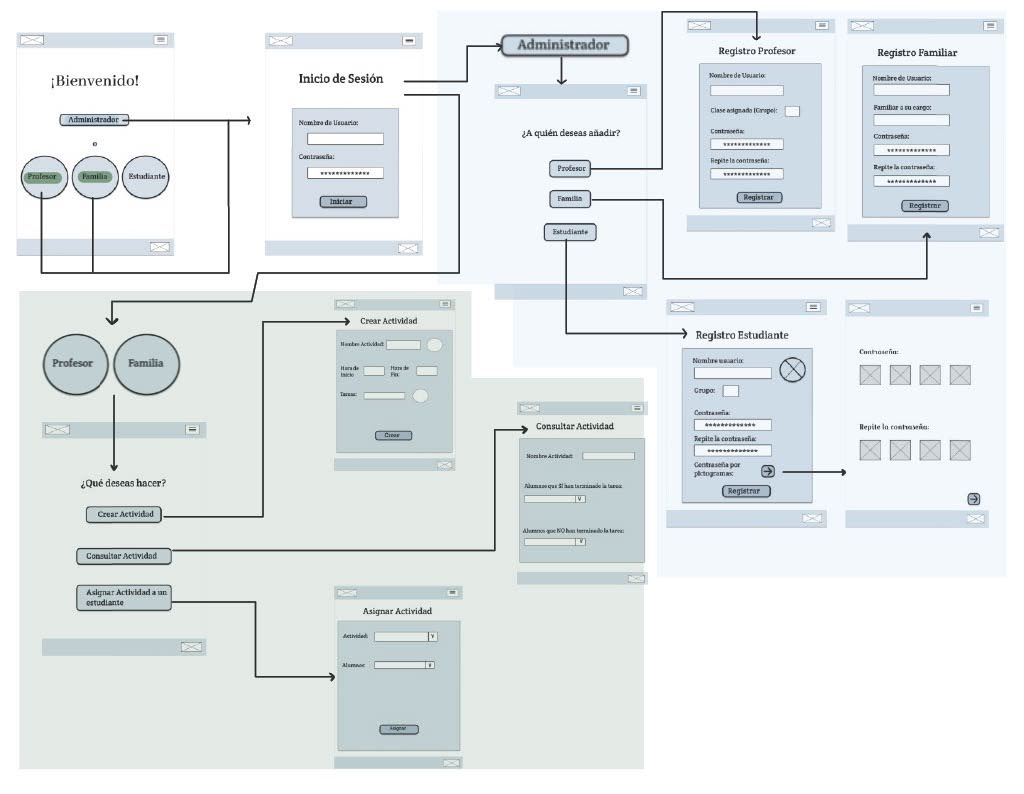
\includegraphics[width=1.2\textwidth]{img/primeraiteracion/esquema_general.png}
    \caption{Esquema general de navegación de la aplicación.}
    \label{fig:esquema_general}
\end{figure}

\begin{figure}[H]
    \centering
     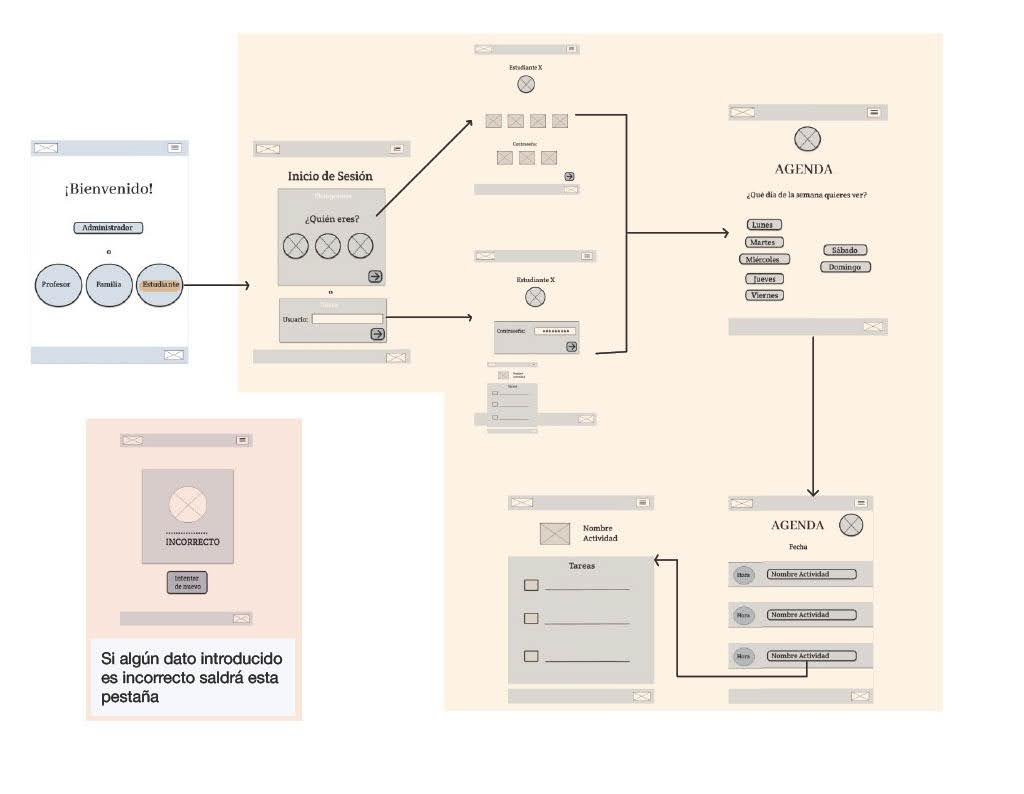
\includegraphics[width=1.2\textwidth]{img/primeraiteracion/esquema_general2.png}
    \caption{Esquema general de navegación de la aplicación.}
    \label{fig:esquema_general2}
\end{figure}
\newpage
En primer lugar, nos encontramos con una pantalla de bienvenida donde debemos elegir el perfil con el que deseamos acceder a la aplicación: Administrador, Profesor, Familia o Estudiante. Dependiendo de la opción escogida, el sistema redirige al usuario a su respectivo inicio de sesión o panel de control.

% ------------ IMAGEN: Pantalla de Bienvenida / Selección de Perfil ------------
\begin{figure}[H]
    \centering
    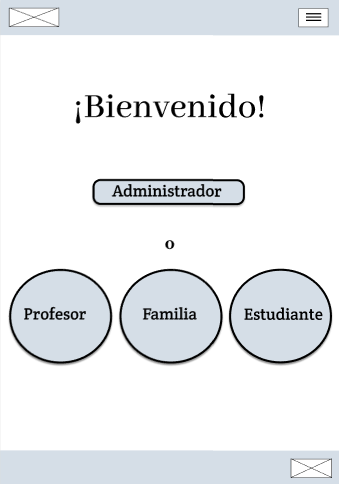
\includegraphics[width=0.6\textwidth]{img/primeraiteracion/pantalla_bienvenida.png}
    \caption{Pantalla de bienvenida y selección de perfil.}
    \label{fig:pantalla_bienvenida}
\end{figure}
\newpage
Si seleccionamos los perfiles de Administrador, Familiar o Profesor, la aplicación redirige a una interfaz de inicio de sesión unificada. En esta pantalla se solicita introducir el Nombre de Usuario y la Contraseña, con un botón para entrar a la aplicación.

% ------------ IMAGEN: Login Administrador, Profesor y Familia ------------
\begin{figure}[H]
    \centering
    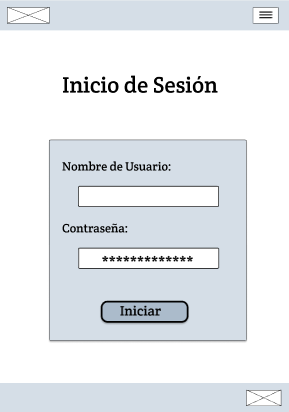
\includegraphics[width=0.8\textwidth]{img/primeraiteracion/login_unificado.png}
    \caption{Interfaz de inicio de sesión unificada para Administrador, Profesor y Familia.}
    \label{fig:login_unificado}
\end{figure}
\newpage
Por otro lado, si seleccionamos el inicio de sesión del estudiante, este ofrece dos alternativas adaptadas a las necesidades del usuario, ya que se puede identificar mediante pictogramas («¿Quién eres?») o introduciendo el nombre de usuario por texto. Dependiendo de la opción escogida, la aplicación redirige a una pantalla u otra para introducir la contraseña: si se entra por pictogramas, la clave se introduce también de forma visual mediante una secuencia de iconos y, si se accede por texto, se utiliza un campo de contraseña tradicional.

% ------------ IMAGEN: Login Estudiante (Texto vs Pictogramas) ------------
\begin{figure}[H]
    \centering
    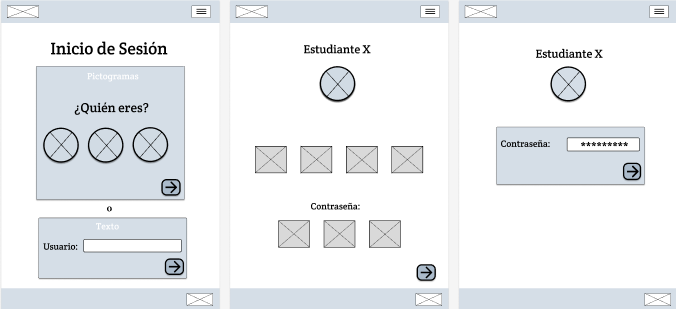
\includegraphics[width=0.6\textwidth]{img/primeraiteracion/login_estudiante.png}
    \caption{Opciones de inicio de sesión para el perfil de Estudiante.}
    \label{fig:login_estudiante}
\end{figure}
\newpage
Si iniciamos la sesión como Administrador, la interfaz muestra una pantalla con la pregunta «¿A quién deseas añadir?», permitiendo escoger entre tres opciones: Profesor, Familia o Estudiante. Dependiendo de la selección, el sistema redirige al usuario hacia el formulario de registro correspondiente para dar de alta al nuevo usuario en la plataforma.

\begin{figure}[H]
    \centering
    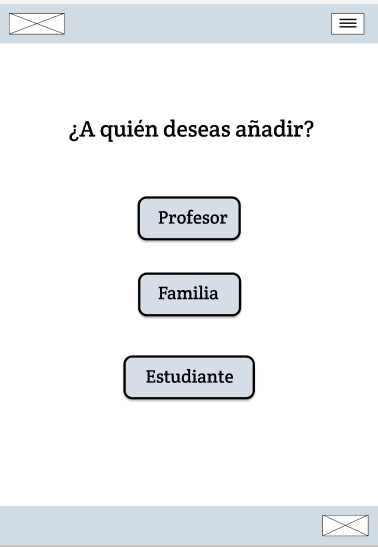
\includegraphics[width=0.6\textwidth]{img/primeraiteracion/interfaz_admin.png}
    \caption{Interfaz de administración para el perfil de Administrador.}
    \label{fig:interfaz_admin}
\end{figure}
\newpage
Si optamos por registrar un Profesor, la pantalla muestra un formulario donde se solicita el nombre de usuario, la clase asignada, la contraseña y su confirmación. De forma similar, si elegimos la opción de Familiar, el formulario solicita el nombre de usuario, el estudiante vinculado al familiar, la contraseña y su correspondiente repetición para validar el registro.

\begin{figure}[H]
    \centering
    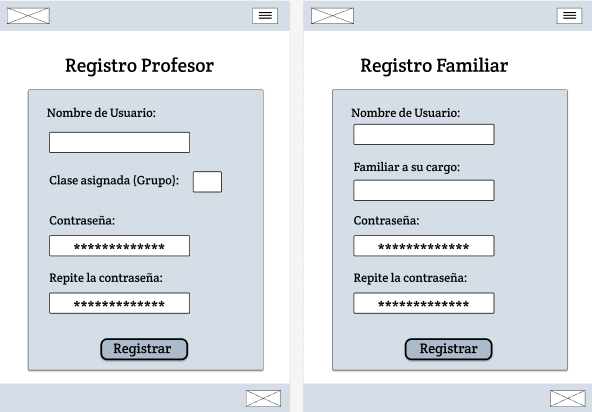
\includegraphics[width=0.8\textwidth]{img/primeraiteracion/registrar_profesor.png}
    \caption{Interfaz de registro de usuarios para los perfiles de Profesor y Familiar.}
    \label{fig:registrar_profesor}
\end{figure}
\newpage
Por otro lado, si elegimos la opción de Estudiante, accedemos a una pantalla de registro donde se solicita el nombre de usuario, el grupo y la contraseña mediante texto. No obstante, para aquellos estudiantes que se comunican o interactúan mejor de forma visual o que lo soliciten, la aplicación incluye la posibilidad de introducir y configurar la contraseña mediante pictogramas, donde de los cuatro pictogramas que se presentan, deberán seleccionar tres (pudiendo ser tres diferentes, tres iguales, dos iguales o la combinación que prefiera para su contraseña).

% ------------ IMAGEN: Formularios de Registro de Usuarios ------------
\begin{figure}[H]
    \centering
    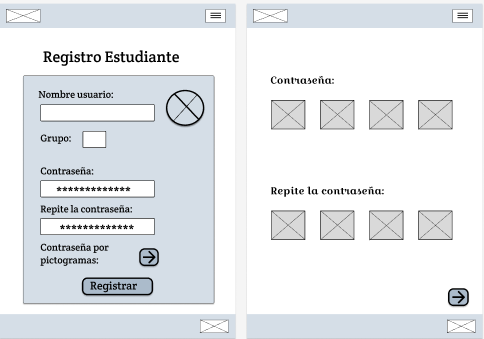
\includegraphics[width=0.8\textwidth]{img/primeraiteracion/registrar_estudiante.png}
    \caption{Interfaz de registro de usuarios para el perfil de Estudiante.}
    \label{fig:registrar_estudiante}
\end{figure}
\newpage
Si iniciamos sesión como Profesor o Familiar, la aplicación muestra una pantalla con la pregunta «¿Qué deseas hacer?». Desde aquí se puede elegir entre tres opciones principales mediante botones: «Crear Actividad», «Consultar Actividad» o «Asignar Actividad a un Estudiante».

% ------------ IMAGEN: Gestión de Actividades (Crear, Consultar y Asignar) ------------
\begin{figure}[H]
    \centering
    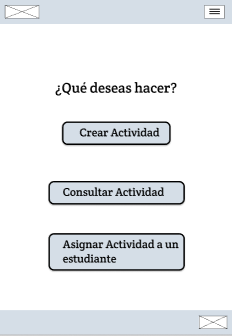
\includegraphics[width=0.6\textwidth]{img/primeraiteracion/gestion_actividades.png}
    \caption{Pantallas de gestión de actividades para Profesor y Familia.}
    \label{fig:gestion_actividades}
\end{figure}
\newpage
Si seleccionamos la opción de Crear Actividad, se despliega un formulario que permite configurar los detalles de la nueva actividad, donde se debe indicar el Nombre de la Actividad y el pictograma asociado, la Hora de Inicio y la Hora de Fin, así como un apartado para añadir las tareas vinculadas a la actividad y un botón de «Crear» para guardar los cambios.
\begin{figure}[H]
    \centering
    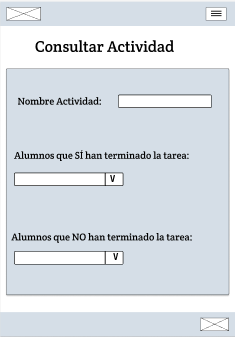
\includegraphics[width=0.6\textwidth]{img/primeraiteracion/crear_actividad.png}
    \caption{Pantallas de creación de actividades.}
    \label{fig:crear_actividad}
\end{figure}
\newpage
Por otro lado, si seleccionamos Consultar Actividad, accedemos a una pantalla de seguimiento que incluye el Nombre de la Actividad, las personas que la han completado y las personas que no. En el caso de los perfiles de Familiar, los listados desplegables de los alumnos que sí han terminado la tarea y de los alumnos que no han terminado la tarea se filtran de forma exclusiva para mostrar únicamente al alumno que tienen asociado a su cargo.
\begin{figure}[H]
    \centering
    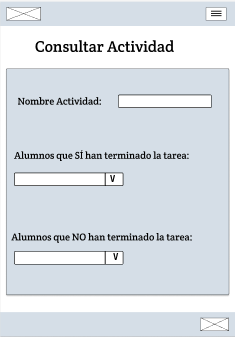
\includegraphics[width=0.6\textwidth]{img/primeraiteracion/consultar_actividad.png}
    \caption{Pantallas de consulta de actividades.}
    \label{fig:consultar_actividad}
\end{figure}
\newpage
Por último, si seleccionamos Asignar Actividad a un estudiante, tenemos dos campos desplegables: uno para seleccionar la Actividad y otro para elegir el Alumno o Alumnos al que se le va a asignar, finalizando con un botón de «Asignar». De igual forma que en «Consultar Actividad», si el usuario que realiza la acción es un Familiar, el desplegable de alumnos se restringe de forma que solo muestra al alumno que tiene a su cargo.
\begin{figure}[H]
    \centering
    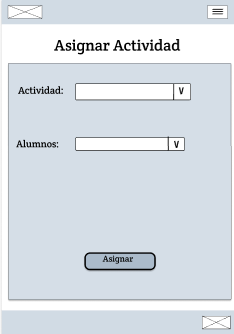
\includegraphics[width=0.6\textwidth]{img/primeraiteracion/asignar_actividad.png}
    \caption{Pantallas de asignación de actividades.}
    \label{fig:asignar_actividad}
\end{figure}
\newpage
Si iniciamos sesión como estudiante, se muestra la pantalla principal de su Agenda, donde se encuentra su imagen de usuario en la parte superior. Bajo el título, se plantea la pregunta «¿Qué día de la semana quieres ver?» y se presentan botones para seleccionar cada uno de los días.
\begin{figure}[H]
    \centering
    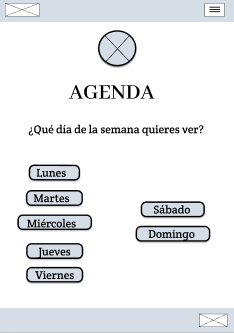
\includegraphics[width=0.6\textwidth]{img/primeraiteracion/panel_agenda.png}
    \caption{Pantalla principal de la Agenda del Estudiante.}
    \label{fig:panel_agenda}
\end{figure}
\newpage
Al pulsar sobre cualquiera de los días de la semana, la aplicación muestra la vista detallada de la Agenda para esa fecha concreta. En esta pantalla se despliega un listado con las actividades programadas, mostrando para cada una de ellas un círculo con la Hora de realización y un cuadro con el Nombre de la Actividad (que podrán ponerse en formato texto o con pictogramas).
\begin{figure}[H]
    \centering
    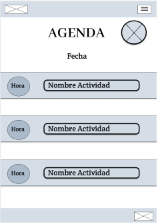
\includegraphics[width=0.6\textwidth]{img/primeraiteracion/vista_detalle_agenda.png}
    \caption{Pantalla principal, diaria y de detalle de tareas para el perfil Estudiante.}
    \label{fig:vista_detalle_agenda}
\end{figure}
\newpage
Al pulsar sobre una actividad específica, se accede a su pantalla de detalle. En la cabecera se muestra el Nombre de la Actividad acompañada de su pictograma asociado. Debajo, en la sección de Tareas, se despliega el listado donde cada elemento puede presentarse mediante texto o pictogramas dependiendo de la configuración del estudiante, incluyendo una casilla cuadrada a la izquierda diseñada para que el alumno pueda marcar la tarea como completada.

% ------------ IMAGEN: Vistas de la Agenda de Estudiante ------------
\begin{figure}[H]
    \centering
    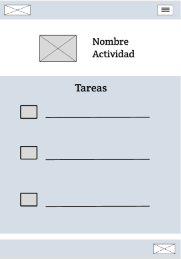
\includegraphics[width=0.6\textwidth]{img/primeraiteracion/detalle_actividad.png}
    \caption{Vista de detalle de una actividad en la Agenda del Estudiante.}
    \label{fig:detalle_actividad}
\end{figure}
\newpage
Para finalizar, la aplicación cuenta con una pantalla de error. En caso de que se introduzca un campo incorrecto en cualquiera de los formularios o procesos (como la contraseña o el nombre de usuario), el sistema redirige a esta interfaz, donde se muestra un icono superior, el texto correspondiente indicando qué campo ha sido incorrecto y un botón de «Intentar de nuevo» para volver a la pantalla anterior.

% ------------ IMAGEN: Pantalla de Error ------------
\begin{figure}[H]
    \centering
    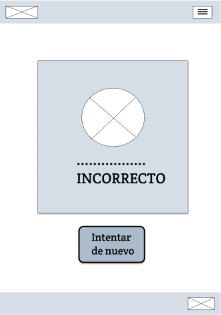
\includegraphics[width=0.6\textwidth]{img/primeraiteracion/pantalla_error.png}
    \caption{Pantalla de error en el sistema.}
    \label{fig:pantalla_error}
\end{figure}

\subsection{Bocetos Base de Datos}
\begin{figure}[H]
    \centering
    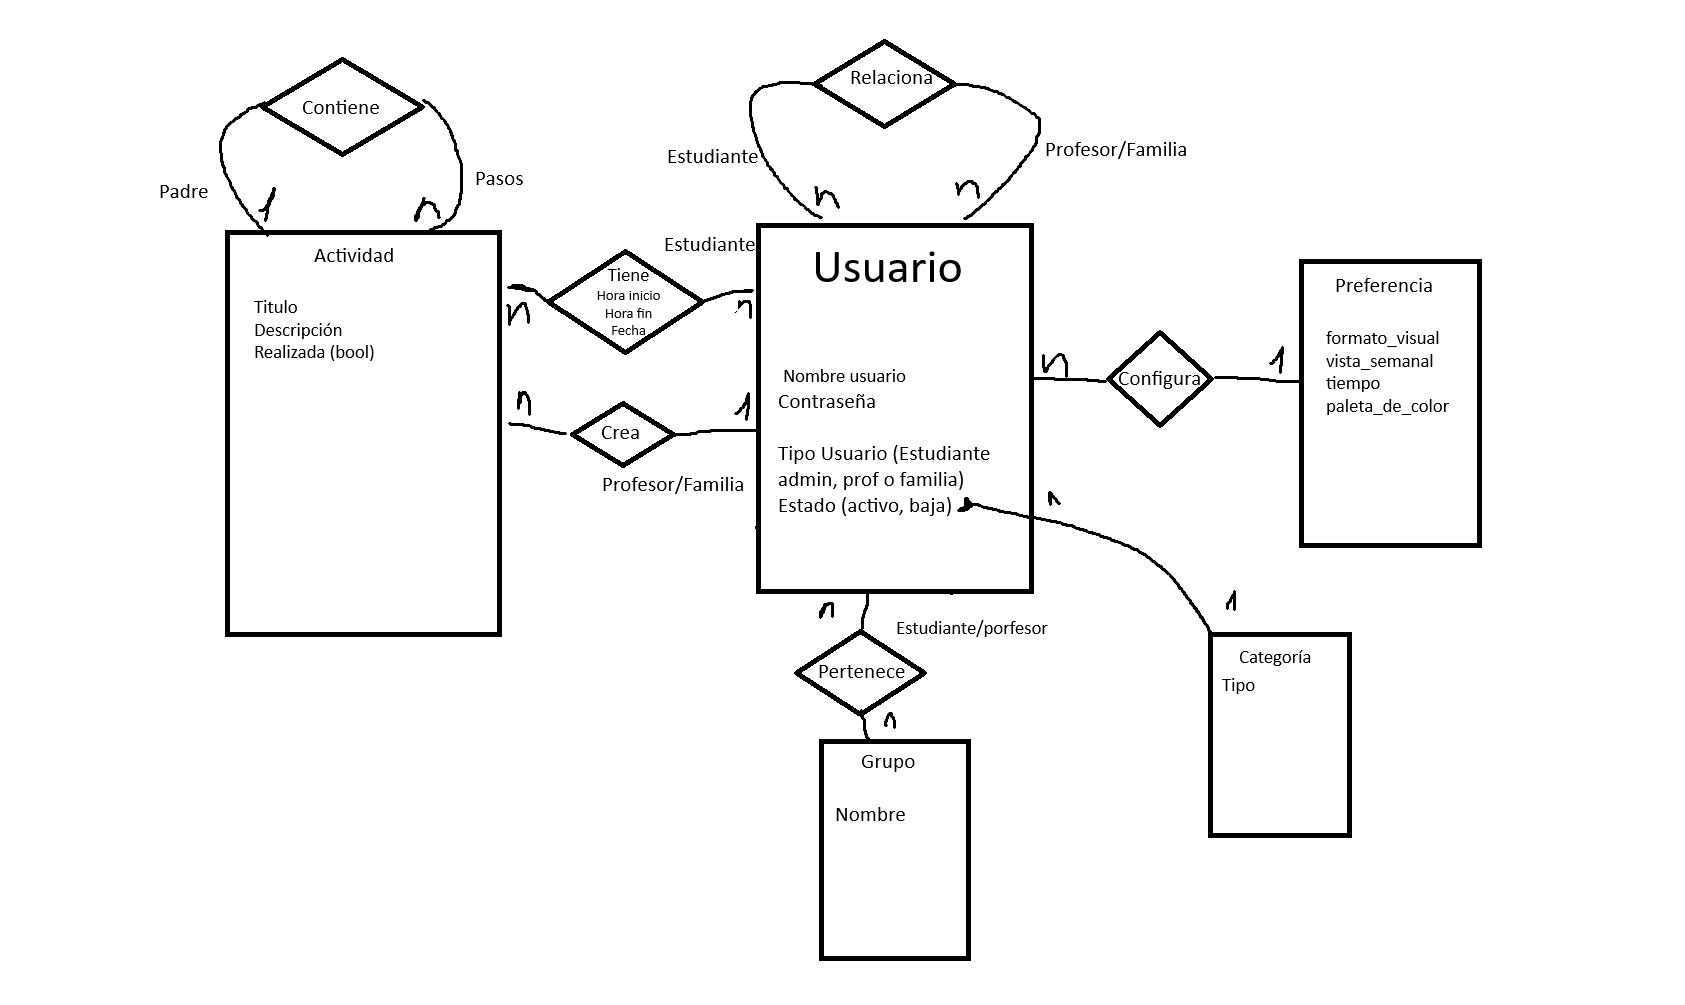
\includegraphics[width=1.2\textwidth]{img/primeraiteracion/bd_boceto.png}
    \caption{Boceto de la Base de Datos.}
    \label{fig:bd_boceto}
\end{figure}



\newpage
\section{Manual de Calidad}

\subsection{Objeto y Alcance del Manual de Calidad}
El presente Manual de Calidad establece los principios, metodologías, métricas y controles que garantizan la calidad del producto final y de la documentación generada durante el desarrollo de la aplicación web \textbf{Doble Agenda}. 

Este plan se aplica de forma continua e integrada a lo largo del ciclo de vida del proyecto (desarrollado bajo la metodología Scrum) y abarca la validación de requisitos de usabilidad y accesibilidad cognitiva, los estándares de código fuente, la trazabilidad documental en \LaTeX{} y el control del trabajo en equipo según las pautas fijadas en el Manual de Coordinación.

\subsection{Criterios y Dimensiones Objetivas de Calidad}

Para asegurar que las entregas cumplan con los estándares exigidos por el equipo y el cliente, se definen métricas objetivas de obligado cumplimiento evaluadas en cada iteración:

\subsubsection{Dimensiones de Calidad para la Documentación (\LaTeX)}
Siguiendo los estándares fijados en la Sección 3.6 del Manual de Coordinación, la documentación debe cumplir con los siguientes criterios:
\begin{itemize}
    \item \textbf{Compilación y Formato Corporativo (100\%):} Todos los documentos deben compilar sin errores ni advertencias graves en \LaTeX{}, incorporando la portada oficial, encabezados y pies de página corporativos con el logotipo de DobleM y la paleta de colores institucional (\texttt{verdeApagado} y \texttt{azulPastelApagado}).
    \item \textbf{Trazabilidad de Requisitos (100\%):} Toda funcionalidad o boceto descrito debe estar explícitamente vinculado a sus códigos de requisitos funcionales (\textsf{RF}), no funcionales (\textsf{RNF}) o de información (\textsf{RI}).
    \item \textbf{Calidad Ortográfica y Terminológica:} Ausencia total de errores ortográficos, garantizando una redacción técnica clara, coherente y precisa en español.
\end{itemize}

\subsubsection{Dimensiones de Calidad para el Código Fuente}
Para el software desarrollado en la arquitectura MVC (PHP, Twig, JavaScript, HTML, CSS y MySQL) bajo Docker, se aplican los estándares definidos en la Sección 3.7:
\begin{itemize}
    \item \textbf{Estándares de Nomenclatura (100\%):} Cumplimiento estricto del formato \texttt{camelCase} para variables y funciones, \texttt{PascalCase} para clases y \texttt{UPPER\_SNAKE\_CASE} para constantes. Los identificadores deben escribirse en inglés y los comentarios explicativos en español.
    \item \textbf{Modularidad y Tamaño de Funciones:} Ninguna función o método del backend o frontend superará las 50 líneas de código para garantizar su mantenibilidad.
    \item \textbf{Reutilización y Duplicación ($<$5\%):} La duplicación del código fuente se mantendrá por debajo del 5\% mediante la modularización de componentes en Twig y funciones globales en PHP/JavaScript.
    \item \textbf{Integridad de la Rama Principal (\texttt{main}):} El código subido a la rama principal del repositorio GitHub debe estar libre de errores sintácticos y permitir el flujo de usuario completo sin fallos en tiempo de ejecución.
\end{itemize}

\subsubsection{Dimensiones de Calidad en Accesibilidad Cognitiva y Usabilidad}
Dado que el destinatario principal es el alumnado con discapacidad intelectual del PTVAL:
\begin{itemize}
    \item \textbf{Carga Cognitiva Limitada (\textsf{RNF1}):} La interfaz no superará los 15 elementos interactivos contextuales por pantalla.
    \item \textbf{Contraste y Lectura Fácil (\textsf{RNF3}, \textsf{RNF9}):} Cumplimiento del nivel AA de WCAG 2.1 (ratio mínimo 4.5:1 para texto normal) e integración obligatoria de la iconografía de ARASAAC con fuentes sin serifa de tamaño mínimo $18\text{px}$.
    \item \textbf{Área Táctil (\textsf{RNF4}):} Los botones y elementos interactivos mantendrán un tamaño mínimo de $44\times44$ píxeles CSS para asegurar su uso en dispositivos de tipo tableta.
\end{itemize}

\subsection{Procedimientos de Control de Calidad durante el Desarrollo}

La supervisión de la calidad no es una etapa final aislada, sino una responsabilidad continua coordinada por la \textbf{Gestora de Calidad} (Minerva Cebrián Marín) y respaldada por todo el equipo mediante las siguientes acciones:

\begin{enumerate}
    \item \textbf{Seguimiento del Tablero Jira:} Verificación del estado real de las historias de usuario y tareas. Ninguna tarea se dará por "Finalizada" si no ha superado las comprobaciones de código/documentación correspondientes.
    \item \textbf{Revisiones Cruzadas (\textit{Peer Review}):} Antes de fusionar solicitudes de extracción (\textit{pull requests}) en GitHub o dar por cerrado un capítulo del documento, se realizará la revisión previa del código o texto por parte de un integrante diferente al autor.
    \item \textbf{Pruebas de Accesibilidad y Emulación:} Validación periódica del diseño adaptativo y táctil mediante herramientas de emulación de dispositivos (Chromium/Safari Device Mode) y verificación de contraste.
    \item \textbf{Gestión y Corrección de Incidencias:} Todo fallo, inconsistencia tipográfica o desviación en los requisitos detectada se registrará formalmente como una incidencia en Jira, asignándole una prioridad para su resolución inmediata dentro de la iteración en curso.
\end{enumerate}

\subsection{Medición del Desempeño y Control de Calidad Interno}
Para asegurar la cohesión del equipo y el cumplimiento de los compromisos adquiridos en el Plan de Dirección, la calidad del trabajo colectivo se auditará bajo los siguientes indicadores:
\begin{itemize}
    \item \textbf{Tasa de Cumplimiento de Tareas ($\ge 85\%$):} Finalización dentro de los plazos estipulados en cada sprint de la planificación.
    \item \textbf{Trazabilidad del Esfuerzo:} Registro individual de horas dedicadas en la herramienta común con un margen de desviación máximo del $15\%$ respecto a lo estimado.
    \item \textbf{Gestión de Estados:} Modificación en tiempo real del estado, fecha de inicio y finalización de cada tarea asignada en Jira.
\end{itemize}

\newpage
\section{Manual de Despliegue, Arquitectura y Especificación de la API}
\label{sec:guia-tecnica-app}

El presente documento constituye la guía técnica oficial para el despliegue del entorno local, la organización del repositorio y la integración entre los subsistemas de \textit{Front-end} y \textit{Back-end}.

% -----------------------------------------------------------------
% SUBSECCIÓN: PREPARACIÓN DEL ENTORNO LOCAL
% -----------------------------------------------------------------
\subsection{Preparación del Entorno y Despliegue con Docker}

El proyecto utiliza contenedores mediante \textbf{Docker Compose} para estandarizar el entorno de desarrollo. Siga las instrucciones correspondientes a su estado inicial.

\subsubsection{Inicialización por primera vez (Instalación limpia)}
Si nunca se ha compilado el entorno ni realizado la descarga del repositorio, ejecute en la terminal desde la carpeta raíz \texttt{app/}:

\begin{quote}
\small\ttfamily
cd app\\
docker compose up
\end{quote}

\subsubsection{Recompilación del entorno (Entorno previamente montado)}
Si ya contaba con el contenedor y se han integrado cambios en la configuración base, fuerce la reconstrucción sin uso de caché:

\begin{quote}
\small\ttfamily
docker compose down\\
docker compose build --no-cache\\
docker compose up -d
\end{quote}

\subsubsection{Instalación del motor de plantillas Twig}
Una vez que el servidor esté en ejecución, instale las dependencias necesarias ejecutando Composer dentro del contenedor:

\begin{quote}
\small\ttfamily
docker compose exec webserver composer require "twig/twig:\^{}3.0"
\end{quote}

\vspace{0.3cm}
\noindent
\colorbox{azulclaro!40}{%
  \parbox{\dimexpr\textwidth-2\fboxsep\relax}{%
    \vspace{6pt}
    \textbf{\color{textoOscuro}Importante (Front-end):} Para poder renderizar plantillas de Twig correctamente, es \textbf{obligatorio} incluir el autoloader de Composer al inicio de cualquier archivo PHP destinado a renderizado:
    
    \vspace{4pt}
    {\small\ttfamily\hspace*{1em}require\_once \_\_DIR\_\_ . '/vendor/autoload.php';}
    \vspace{4pt}
  }%
}
\vspace{0.3cm}

\vspace{0.5cm}
\subsubsection{Despliegue e Importación de la Base de Datos}
Para mantener sincronizado el esquema de la base de datos con los últimos cambios de \textit{Back-end}, siga el siguiente procedimiento:

\begin{enumerate}
    \item Asegúrese de que el servidor está activo y acceda a \textbf{phpMyAdmin} en su navegador mediante \url{http://localhost/phpmyadmin}.
    \item En el panel izquierdo, busque la base de datos \texttt{agenda}. 
    \item \textbf{Si ya existe:} Selecciónela, diríjase a la pestaña \textit{Operaciones} y ejecute la opción \textbf{Eliminar la base de datos (DROP)}.
    \item \textbf{Creación de BD limpia:} Haga clic en \textit{Nueva} en el menú izquierdo, introduzca el nombre \texttt{agenda} y pulse \textit{Crear}.
    \item \textbf{Importación del Backup:} Seleccione la base de datos \texttt{agenda}, acuda a la pestaña superior \textit{Importar}, cargue el archivo situado en:
    \begin{center}
        \texttt{app/BD Backup/agenda.sql}
    \end{center}
    y confirme la operación con el botón \textit{Importar}.
\end{enumerate}

% -----------------------------------------------------------------
% SUBSECCIÓN: ESTRUCTURA DE ARCHIVOS Y DIRECTORIOS
% -----------------------------------------------------------------
\newpage
\subsection{Arquitectura y Estructura del Proyecto}

Toda la aplicación se encuentra encapsulada dentro del directorio \texttt{app/}. A continuación se especifica la responsabilidad de cada subdirectorio y su equipo encargado:

\begin{table}[H]
\centering
\small
\rowcolors{2}{white}{azulclaro!30}
\begin{tabularx}{\textwidth}{l c X}
\toprule
\rowcolor{azulPastelApagado}
\textbf{\color{textoOscuro}Directorio / Archivo} & \textbf{\color{textoOscuro}Responsable} & \textbf{\color{textoOscuro}Descripción y Propósito} \\
\midrule
\texttt{app/api/} & Back-end & Endpoints PHP invocados vía JavaScript/Fetch para responder datos de la BD en formato JSON. \\
\texttt{app/assets/} & Compartido & Recursos globales (hojas de estilo estáticas base, favicon, imágenes globales). \\
\texttt{app/BD Backup/} & Back-end & Contiene los scripts SQL (\texttt{agenda.sql}) con el estado más reciente de la BD. \\
\texttt{app/css/} & Front-end & Estilos CSS específicos de la aplicación web. \\
\texttt{app/js/} & Front-end & Archivos JavaScript con la lógica de interactividad, animaciones y peticiones asíncronas (\textit{Fetch}). \\
\texttt{app/services/} & Back-end & Servicios del sistema (gestores de sesión, controladores de conexión a la BD). \\
\texttt{app/templates/} & Front-end & Plantillas Twig y vistas parciales HTML (headers, footers, componentes visuales). \\
\texttt{app/utils/} & Back-end & Funciones auxiliares y glosario de utilidades para consultas a la base de datos. \\
\texttt{app/vendor/} & Sistema & Librerías y autoloader gestionados por Composer (\textbf{no modificar}). \\
\texttt{app/renders/} & Front-end & \textit{(Opcional)} Directorio recomendado para organizar los controladores PHP de renderizado de vistas. \\
\bottomrule
\end{tabularx}
\caption{Organización del directorio principal de la aplicación.}
\end{table}

\paragraph{Archivos del Entorno Base (No modificar)}
Los archivos \texttt{index.php}, \texttt{phpinfo.php}, \texttt{test\_db.php}, \texttt{test\_db\_pdo.php}, \texttt{composer.json} y \texttt{composer.lock} pertenecen a la infraestructura LAMP y gestores de paquetes. No deben editarse salvo requerimiento expreso del equipo.

% -----------------------------------------------------------------
% SUBSECCIÓN: GUÍA DE INTEGRACIÓN Y ENDPOINTS DE LA API
% -----------------------------------------------------------------
\newpage
\subsection{Especificación de la API HTTP / JSON}

El flujo de información en la plataforma sigue el patrón cliente-servidor asíncrono. Un archivo de renderizado invoca la plantilla Twig; esta carga un script JS que consulta la API pública enviando y recibiendo estructuras JSON.

\subsubsection{Estándar de Respuesta JSON}
Todos los endpoints ubicados en \texttt{app/api/} devuelven una respuesta con la siguiente estructura base:

\begin{quote}
\small\ttfamily
\{\\
\ \ "success": true,\ \ \ // Booleano: indica si la operación fue exitosa\\
\ \ "code": 0,\ \ \ \ \ \ \ \ // Entero: código de estado/error específico\\
\ \ "message": "..."\ \ // String: descripción legible del resultado o fallo\\
\}
\end{quote}

\subsubsection{Catálogo de Endpoints Disponibles}

\begin{enumerate}
    \item \texttt{crear\_estudiante.php}
    \begin{itemize}
        \item \textbf{Función:} Registra un nuevo perfil de estudiante.
        \item \textbf{Parámetros GET/POST:} \texttt{name} (Nombre de usuario), \texttt{pass} (Contraseña).
        \item \textbf{Códigos posibles:} \texttt{0} (Éxito), \texttt{100} (Falta parámetro), \texttt{200} (Usuario ya existe).
    \end{itemize}

    \item \texttt{crear\_profesor.php}
    \begin{itemize}
        \item \textbf{Función:} Registra un nuevo perfil de docente.
        \item \textbf{Parámetros GET/POST:} \texttt{name} (Nombre de usuario), \texttt{pass} (Contraseña).
        \item \textbf{Códigos posibles:} \texttt{0}, \texttt{100}, \texttt{200}.
    \end{itemize}

    \item \texttt{crear\_familiar.php}
    \begin{itemize}
        \item \textbf{Función:} Registra un perfil para tutores o familiares.
        \item \textbf{Parámetros GET/POST:} \texttt{name} (Nombre de usuario), \texttt{pass} (Contraseña).
        \item \textbf{Códigos posibles:} \texttt{0}, \texttt{100}, \texttt{200}.
    \end{itemize}

    \item \texttt{crear\_pertenece.php}
    \begin{itemize}
        \item \textbf{Función:} Asigna la pertenencia de un usuario a un grupo concreto.
        \item \textbf{Parámetros GET/POST:} \texttt{user} (Usuario), \texttt{group} (Grupo destino).
        \item \textbf{Códigos posibles:} \texttt{0}, \texttt{100}, \texttt{201} (Asignación previa), \texttt{300}, \texttt{301} (Grupo no existe), \texttt{400}.
    \end{itemize}

    \item \texttt{crear\_asociacion.php}
    \begin{itemize}
        \item \textbf{Función:} Asocia a un estudiante con su responsable legal o docente.
        \item \textbf{Parámetros GET/POST:} \texttt{student} (Estudiante), \texttt{responsible} (Profesor/Familiar).
        \item \textbf{Códigos posibles:} \texttt{0}, \texttt{100}, \texttt{202} (Asociación existente), \texttt{300}, \texttt{400}.
    \end{itemize}

    \item \texttt{consultar\_responsable\_asociado\_estudiante.php}
    \begin{itemize}
        \item \textbf{Función:} Verifica la vinculación de responsabilidad entre un estudiante y un tutor/docente.
        \item \textbf{Parámetros GET/POST:} \texttt{student}, \texttt{responsible}.
        \item \textbf{Códigos posibles:} \texttt{0} (Asociado), \texttt{1} (No asociado / \texttt{success: false}), \texttt{100}.
    \end{itemize}

    \item \texttt{login\_estudiante.php}
    \begin{itemize}
        \item \textbf{Función:} Valida credenciales e inicia sesión para la cuenta de estudiante.
        \item \textbf{Parámetros GET/POST:} \texttt{name}, \texttt{pass}.
        \item \textbf{Códigos posibles:} \texttt{0}, \texttt{100}, \texttt{203} (Password incorrecta), \texttt{300}, \texttt{400}, \texttt{401} (Cuenta inactiva).
    \end{itemize}

    \item \texttt{consultar\_agenda\_estudiante.php}
    \begin{itemize}
        \item \textbf{Función:} Recupera la agenda de actividades personalizada del alumno en sesión.
        \item \textbf{Parámetros Opcionales:} \texttt{view} (\texttt{'daily'} por defecto o \texttt{'weekly'}), \texttt{date} (\texttt{YYYY-MM-DD}), \texttt{startDate}, \texttt{endDate}.
        \item \textbf{Códigos posibles:} \texttt{0} (Devuelve array de tareas o array vacío si no hay datos), \texttt{400} (Sesión inválida/no autorizada).
    \end{itemize}

    \item \texttt{consultar\_actividad\_estudiante.php}
    \begin{itemize}
        \item \textbf{Función:} Extrae la información detallada de una tarea (estado actual y desglose de subtareas).
        \item \textbf{Parámetros GET/POST:} \texttt{id\_actividad} (Identificador único).
        \item \textbf{Códigos posibles:} \texttt{0}, \texttt{100}, \texttt{300}, \texttt{400}.
    \end{itemize}
\end{enumerate}

% -----------------------------------------------------------------
% SUBSECCIÓN: DICCIONARIO DE CÓDIGOS DE ERROR
% -----------------------------------------------------------------
\subsubsection{Diccionario de Códigos de Respuesta}

\begin{table}[H]
\centering
\small
\rowcolors{2}{white}{azulclaro!30}
\begin{tabularx}{\textwidth}{c c X}
\toprule
\rowcolor{azulPastelApagado}
\textbf{\color{textoOscuro}Código} & \textbf{\color{textoOscuro}Estado} & \textbf{\color{textoOscuro}Descripción e Interpretación} \\
\midrule
\textbf{0} & Éxito & Operación realizada correctamente. \\
\textbf{1} & Éxito Evaluatorio & Consulta completada pero la condición resulta falsa (\texttt{success: false}). \\
\textbf{100} & Error Parámetros & Falta una o varias variables requeridas para procesar la petición. \\
\textbf{200} & Error Duplicado & El nombre de usuario especificado ya se encuentra registrado. \\
\textbf{201} & Error Duplicado & La relación de pertenencia a grupo ya existe. \\
\textbf{202} & Error Duplicado & La asociación entre estudiante y responsable ya está registrada. \\
\textbf{203} & Error Credenciales & La contraseña proporcionada no es válida. \\
\textbf{300} & No Encontrado & El recurso solicitado (usuario, actividad, etc.) no existe en el sistema. \\
\textbf{301} & No Encontrado & El grupo especificado no existe. \\
\textbf{400} & No Autorizado & Permisos insuficientes o ausencia de sesión activa. \\
\textbf{401} & Cuenta Bloqueada & El usuario se encuentra dado de baja o inactivo. \\
\bottomrule
\end{tabularx}
\caption{Codificación estándar de respuestas de la API.}
\end{table}


